\chapter{Architettura di un Sistema Operativo}

In un sistema operativo è molto importante separare le \textit{policy} dai \textit{meccanismi}. I meccanismi sono le funzionalità che il sistema operativo mette a disposizione, mentre le \textit{policy} sono le regole che il sistema operativo segue per decidere come utilizzare i meccanismi.

\paragraph{Principi di progettazione} Il principio di progettazione di un sistema operativo è quello di \texttt{KISS} (\textit{Keep It Small and Simple}) usato per ottimizzare al meglio le \textit{performance} implementando solo lo stretto necessario. Altro principio è il \texttt{POLP} (\textit{Principle of Least Privilege}), ovvero dare il minimo dei privilegi necessari ad ogni componente per svolgere il proprio compito. Quest'ultimo principio è molto importante per garantire affidabilità e sicurezza.

\section{Tipi di architetture}
    \subsubsection{Sistemi monoblocco}
        Nei sistemi monoblocco non è presente una gerarchia tra i vari livelli del sistema operativo. Questo tipo di architettura è molto semplice e consiste in un unico strato \textit{software} tra l'utente ed l'\textit{hardware} del sistema. Le componenti sono dunque tutte allo stesso livello permettendo una comunicazione diretta tra l'utente e l'\textit{hardware}. Questo tipo di architettura è molto semplice e veloce, ma il codice risulta interamente dipendente dall'architettura ed è distribuito su tutto il sistema operativo. Inoltre per testare ed eseguire il \textit{debugging} di un singolo componente è necessario analizzare l'intero sistema operativo.
    \subsubsection{Sistemi a struttura semplice}
        Nei sistemi a struttura semplice è presente una piccola gerarchia, molto flessibile, tra i vari livelli del sistema operativo. Questo tipo di architettura mira ad una riduzione dei costi di sviluppo ed di manutenzione del sistema operativo. Non avendo una struttura ben definita, i componenti possono comunicare tra loro in modo diretto. Questo tipo di architettura è molto flessibile e permette di avere un sistema operativo molto piccolo e veloce come \texttt{MS-DOS} o \texttt{UNIX} originale.
        \paragraph{\texttt{MS-DOS}} Il sistema operativo \texttt{MS-DOS} è un sistema operativo a struttura semplice, molto piccolo e veloce. Questo sistema operativo è pensato per fornire il maggior numero di funzionalità in uno spazio ridotto. Infatti non sussistono suddivisioni in moduli, ed le interfacce e livelli non sono ben definiti. È infatti possibile accedere direttamente alle \textit{routine} del sistema operativo ed non è prevista la \textit{dual mode}.
        \paragraph{\texttt{UNIX} (Originale)} Struttura semplice limitata dalle poche funzionalità disponibili all'epoca in materia di \textit{hardware}, con un \textit{kernel} molto piccolo e veloce il quale scopo è risiedere tra l'interfaccia delle \textit{system call} e l'\textit{hardware}. Questo sistema operativo è stato progettato per essere molto flessibile e fornisce: \textit{File System}, \textit{Scheduling} della \texttt{CPU}, gestione della memoria e molto altro.
        \begin{figure}[H]
            \centering
            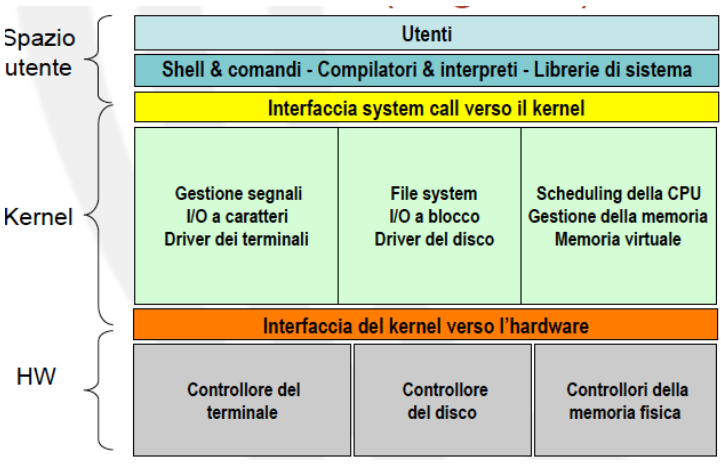
\includegraphics[width=0.6\textwidth]{03/unixOriginal.png}
            \caption{Struttura di \texttt{UNIX} originale}
        \end{figure}
    \subsubsection{Sistema a livelli}
        Nei sistemi operativi organizzati a livelli gerarchici l'interfaccia utente risiede al livello più altro mentre l'\textit{hardware} dal lato opposto. Ogni livello intermedio può solo usare funzioni fornite dal livello inferiore ed offrire funzionalità al livello superiore. Principale vantaggio di questa architettura è la modularità, infatti ogni livello può essere sviluppato e testato indipendentemente dagli altri. Questo tipo di architettura, d'altronde non è priva di svantaggi, infatti diventa difficile definire in modo approssimato gli strati, l'efficienza decresce in quanto ogni singolo strato aggiunge un costo di \textit{overhead} ed le funzionalità dipendenti dal'\textit{hardware} sono sparse su più livelli.
        \paragraph{\texttt{THE}} Il sistema operativo \texttt{THE} è un sistema d'uso accademico ed è il primo sistema operativo a struttura a livelli. Questo \texttt{SO} consiste in un insieme di processo che cooperano tra di loro usando la tecnica dei ``semafori'' per la sincronizzazione. \begin{figure}[H]
            \centering
            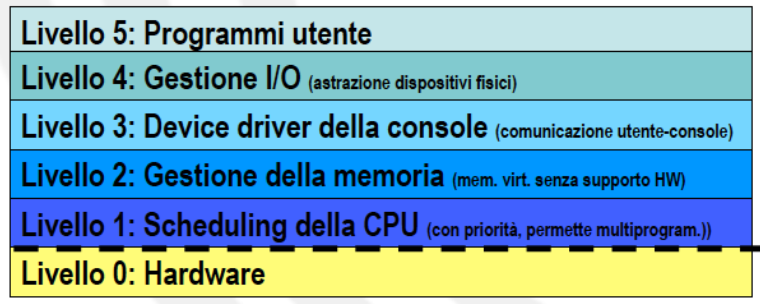
\includegraphics[width=0.4\textwidth]{03/the.png}
            \caption{Struttura di \texttt{THE}}
        \end{figure}
    
    \subsubsection{Sistemi basati su \textit{Kernel}}
        I sistemi di questo genere hanno due soli livelli: i servizi \textit{kernel} e quelli non-\textit{kernel} (o \textit{utente}). Il \textit{file system} è un esempio di servizio non-\textit{kernel}. Questo tipo di architettura è molto diffuso in quanto il ridotto e ben definito numero di livelli ne permette una facile implementazione e manutenzione, spesso però questo sistema può risultare troppo rigido e non adatto a tutti i tipi di applicazioni, oltre alla totale assenza di regole organizzative per le parti del \texttt{SO} al di fuori del \textit{kernel}.
    \subsubsection{\textit{Micro-kenrel}} 
        Questo tipo di \textit{kernel} è molto piccolo e fornisce solo i servizi essenziali per il funzionamento del sistema operativo. Tutte le altre funzionalità sono implementate come processi utente. Un esempio di ciò è \texttt{seL4} un \textit{kernel} \textit{open source} che implementa un \textit{micro-kernel} e fornisce un'interfaccia per la gestione della memoria, dei processi e della comunicazione tra processi. \texttt{SeL4} è matematicamente verificato e privo di bug rispetto alle sue specifiche di forte sicurezza 
    \subsubsection{\textit{Virtual Machine}}
        L'architettura a \texttt{VM} è una estremizzazione dell'approccio a più livelli di \texttt{IBM} (1972), questo è pensato per offrire un sistema di \textit{timesharing} ``multiplo'' dove il sistema operativo viene eseguito su una \texttt{VM} ed questa dà illusione di processi multipli, ma nella realtà ognuno di questi è in esecuzione sul proprio \texttt{HW}. In questo paradigma sono possibili più \texttt{SO} in una unica macchina. 
        \begin{figure}[H]
            \centering
            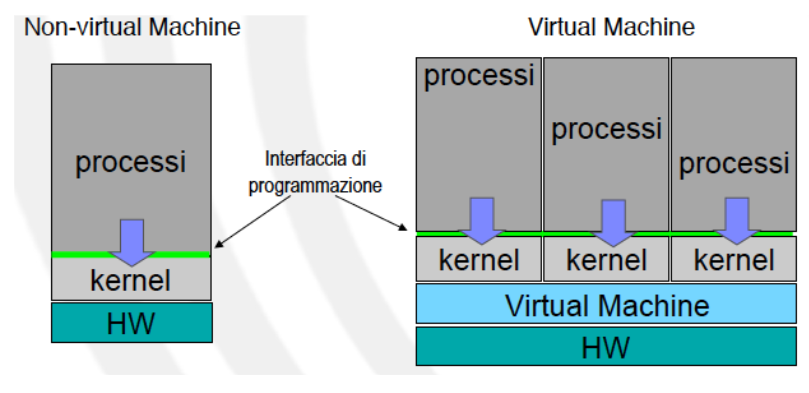
\includegraphics[width=0.4\textwidth]{03/diffVmNoVm.png}
            \caption{Differenze tra una macchina senza e con \texttt{VM}}
        \end{figure}
        Come è possibile notare ogni singolo processo è separato ed possiede il proprio \textit{kernel}. Vengono quindi separata la multiprogrammazione ed la presentazione.
        \paragraph{Tipo di \textit{Hypervisor}}
            \begin{itemize}
                \item \textbf{Tipo 1} (\textit{Bare Metal}): Questo tipo di \textit{Hypervisor} è installato direttamente sul'\textit{hardware} e non necessita di un sistema operativo ospite. Questo tipo di \textit{Hypervisor} è molto veloce e sicuro, ma è molto complesso da installare e configurare.
                \item \textbf{Tipo 2} (\textit{Hosted}): Questo tipo di \textit{Hypervisor} è installato sopra un sistema operativo ospite. Questo tipo di \textit{Hypervisor} è molto più semplice da installare e configurare rispetto al tipo 1, ma è più lento e meno sicuro, inoltre è possibile avere problemi di compatibilità tra il sistema operativo ospite e il \textit{Hypervisor}.
            \end{itemize}
        \paragraph{\textit{Monolithic} vs \textit{Micro-kernel} \texttt{VM}}
            Prima di fare una distinzione tra i due tipi di \texttt{VM} è necessario dire che entrambi rientrano nel tipo 1 di \textit{Hypervisor} e dunque tutti i \texttt{SO} sono eseguiti direttamente sul'\textit{hardware} virtualizzato.
            \begin{itemize}
                \item \textbf{\textit{Monolithic}}: Questo tipo di \texttt{VM} è molto simile ad un sistema operativo tradizionale, infatti ogni \textit{VM} è un processo separato che esegue il proprio \textit{kernel}. Questo tipo di \texttt{VM} è molto veloce, ma è molto complesso da implementare e mantenere.
                \item \textbf{\textit{Micro-kernel}}: Questo tipo di \texttt{VM} è molto simile ad un sistema operativo a \textit{micro-kernel}, infatti il \textit{kernel} della \texttt{VM} fornisce solo i servizi essenziali per il funzionamento del sistema operativo. Tutte le altre funzionalità sono implementate come processi utente. Questo tipo di \texttt{VM} è molto più semplice da implementare e mantenere rispetto al tipo 1, ma è più lento e meno sicuro.
            \end{itemize}
        \paragraph{Vantaggi - Svantaggi}
            Principale vantaggio di questo tipo di architettura è la completa protezione del sistema, infatti ogni \texttt{SO} è separato e non può accedere alle risorse degli altri \texttt{SO}. Inoltre è possibile avere più \texttt{SO} in una sola macchina andando ad ottimizzare le risorse e ridurre i costi di sviluppo di un sistema operativo, oltre ad aumentare la portabilità delle applicazioni. Principale svantaggio riguardano le prestazioni del sistema, infatti ogni \texttt{SO} è eseguito su una \texttt{VM} e questo può portare ad un aumento dei tempi di esecuzione delle applicazioni. Inoltre è necessario avere gestire una \textit{dual-mode} virtuale e non è possibile avere un sistema operativo in tempo reale, inoltre il fatto che una \texttt{VM} non possa accedere alle altre \texttt{VM} può portare ad un aumento dei costi di sviluppo e manutenzione del sistema.
    \subsubsection{Sistemi \textit{client-server}}
        Poco diffusi ai giorni nostri, i sistemi \textit{client-server} sono basati su un'architettura a due livelli: il \textit{client} e il \textit{server}. Questo sistema di basa sull'idea che il codice del sistema operativo vada portato sul livello superiore (il \textit{client}) e il \textit{server} rimanga molto piccolo e veloce andando solo a fornire i servizi essenziali per il funzionamento del sistema operativo ed la comunicazione tra il \textit{client} e l'\textit{hardware}. Questo tipo di architettura si presta bene per sistemi distribuiti.
\section{Implementazione di un \texttt{SO}}
    I sistemi operativi sono tradizionalmente scritti in linguaggio \textit{assembler} anche se è possibile scriverli in linguaggi di alto livello, come \texttt{C} o \texttt{C++}. La scrittura di un sistema operativo in linguaggio di alto livello permette di avere una implementazione molto rapida oltre ad aumentarne la compattezza e la mantienebilità. Inoltre è possibile avere una maggiore portabilità del sistema operativo, in quanto è possibile compilare il codice sorgente su più architetture. Tuttavia la scrittura di un sistema operativo in linguaggio di alto livello può portare ad un aumento dei tempi di esecuzione delle applicazioni e ad un aumento dei costi di sviluppo e manutenzione del sistema operativo. 